
\section{Ejercicio 1}


\subsection{Desarrollo}
Sabiendo que la tarea solamente se dedica a bloquearse una cantidad n de veces y con una duración al azar entre bmin y bmax, lo que hacemos para resolver este ejercicio es 
simplemente conseguirnos un número aleatorio n veces. Para esto usamos la función de c++ rand(), aclarando que queremos que los valores se encuentren entre los pedidos.

\subsection{Experimentación}
Para cumplir con lo pedido en el ejercicio utilizaremos el lote de tareas loteEj1.tsk, la representación del mismo usando la política FCFS es la siguiente:


\begin{figure}[H]
  \centering
    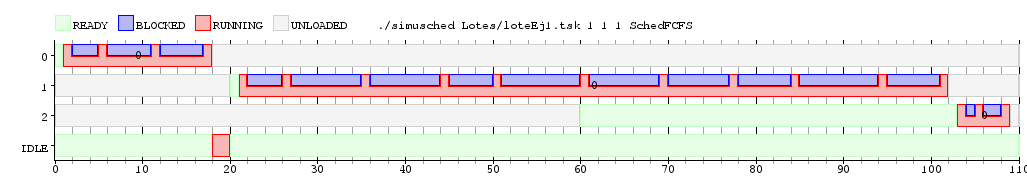
\includegraphics[width=1.1\textwidth]{imagenes/Ex1Ej1.png}
  \caption{loteEj1.tsk con FCFS}
\end{figure}

Con este gráfico podemos ver como, para cada una de las tres tareas, van apareciendo varias llamadas bloqueantes de una duración diferente las unas de las otras. Considerando 
que la cantidad para cada una (especificada por el primer parámetro, n) es correcta y que el tiempo de las llamadas está entre los elegidos, podemos decir que el algoritmo es correcto.

\begin{figure}[H]
  \centering
    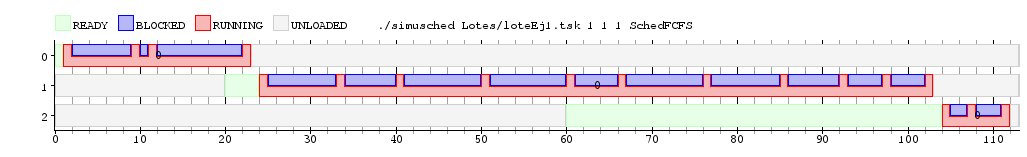
\includegraphics[width=1.1\textwidth]{imagenes/Ex2Ej1.png}
  \caption{loteEj1.tsk con FCFS segundo intento}
\end{figure}

Ejecutamos, por segunda vez, en las mismas condiciones para mostrar como varían los tiempos de los bloqueos.

\begin{figure}[H]
  \centering
    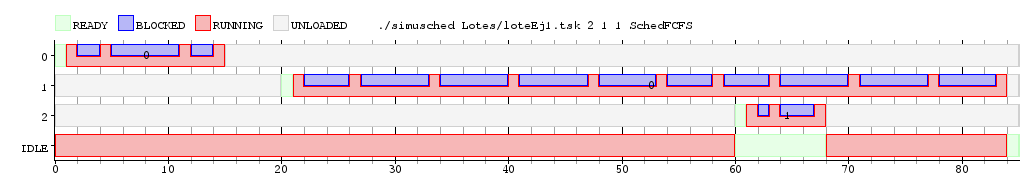
\includegraphics[width=1.1\textwidth]{imagenes/Ex3Ej1.png}
  \caption{loteEj1.tsk con FCFS con dos cores}
\end{figure}

Por último lo hacemos con dos cores, para mostrar como se comporta. 